\documentclass[letterpaper,10pt,conference]{template/ieeeconf}
\IEEEoverridecommandlockouts
\overrideIEEEmargins
\usepackage{amsmath,amssymb,graphicx,booktabs,multirow,url,xcolor}
\usepackage[hidelinks]{hyperref}
\usepackage{flushend}
\graphicspath{{figures/}}
\newcommand{\method}{WA-FGNG}
\newcommand{\R}{\mathbb{R}}
\newcommand{\placeholder}[1]{\textcolor{red}{#1}}
\title{World-Anchored Foveated Growing Neural Gas\\with Bounded Multi-View Replay}
\author{Anonymous authors}
\newcommand{\DeskCameraSeen}{62.80}
\newcommand{\DeskCameraHistory}{86.36}
\newcommand{\DeskCameraFocus}{57.36}
\newcommand{\DeskCameraPeriphery}{63.32}
\newcommand{\DeskCameraCurrent}{9.62}
\newcommand{\DeskCameraEdge}{16.99}
\newcommand{\DeskCameraTime}{1.60}
\newcommand{\DeskCameraNodes}{222}
\newcommand{\DeskWorldSeen}{62.61}
\newcommand{\DeskWorldHistory}{85.26}
\newcommand{\DeskWorldFocus}{56.29}
\newcommand{\DeskWorldPeriphery}{63.21}
\newcommand{\DeskWorldCurrent}{11.38}
\newcommand{\DeskWorldEdge}{3.89}
\newcommand{\DeskWorldTime}{1.33}
\newcommand{\DeskWorldNodes}{170}
\newcommand{\DeskMemorySeen}{10.44}
\newcommand{\DeskMemoryHistory}{11.55}
\newcommand{\DeskMemoryFocus}{5.93}
\newcommand{\DeskMemoryPeriphery}{10.64}
\newcommand{\DeskMemoryCurrent}{10.10}
\newcommand{\DeskMemoryEdge}{5.58}
\newcommand{\DeskMemoryTime}{2.76}
\newcommand{\DeskMemoryNodes}{256}
\newcommand{\DeskUniformSeen}{10.07}
\newcommand{\DeskUniformHistory}{11.17}
\newcommand{\DeskUniformFocus}{7.43}
\newcommand{\DeskUniformPeriphery}{10.20}
\newcommand{\DeskUniformCurrent}{9.61}
\newcommand{\DeskUniformEdge}{5.59}
\newcommand{\DeskUniformTime}{2.75}
\newcommand{\DeskUniformNodes}{256}
\newcommand{\DeskDblSeen}{9.61}
\newcommand{\DeskDblHistory}{10.14}
\newcommand{\DeskDblFocus}{7.44}
\newcommand{\DeskDblPeriphery}{9.69}
\newcommand{\DeskDblCurrent}{8.99}
\newcommand{\DeskDblEdge}{4.86}
\newcommand{\DeskDblTime}{2.46}
\newcommand{\DeskDblNodes}{256}
\newcommand{\DeskFpsSeen}{11.03}
\newcommand{\DeskFpsHistory}{11.27}
\newcommand{\DeskFpsFocus}{11.01}
\newcommand{\DeskFpsPeriphery}{11.04}
\newcommand{\DeskFpsCurrent}{10.47}
\newcommand{\DeskFpsTime}{1.58}
\newcommand{\DeskFpsNodes}{256}
\newcommand{\XyzCameraSeen}{57.47}
\newcommand{\XyzCameraHistory}{90.50}
\newcommand{\XyzCameraFocus}{10.55}
\newcommand{\XyzCameraPeriphery}{60.90}
\newcommand{\XyzCameraCurrent}{9.81}
\newcommand{\XyzCameraEdge}{9.90}
\newcommand{\XyzCameraTime}{1.53}
\newcommand{\XyzCameraNodes}{224}
\newcommand{\XyzWorldSeen}{60.66}
\newcommand{\XyzWorldHistory}{92.19}
\newcommand{\XyzWorldFocus}{10.33}
\newcommand{\XyzWorldPeriphery}{64.32}
\newcommand{\XyzWorldCurrent}{13.00}
\newcommand{\XyzWorldEdge}{4.86}
\newcommand{\XyzWorldTime}{1.44}
\newcommand{\XyzWorldNodes}{201}
\newcommand{\XyzMemorySeen}{9.22}
\newcommand{\XyzMemoryHistory}{11.38}
\newcommand{\XyzMemoryFocus}{4.46}
\newcommand{\XyzMemoryPeriphery}{9.57}
\newcommand{\XyzMemoryCurrent}{6.67}
\newcommand{\XyzMemoryEdge}{4.53}
\newcommand{\XyzMemoryTime}{2.70}
\newcommand{\XyzMemoryNodes}{256}
\newcommand{\XyzUniformSeen}{8.47}
\newcommand{\XyzUniformHistory}{10.11}
\newcommand{\XyzUniformFocus}{5.47}
\newcommand{\XyzUniformPeriphery}{8.70}
\newcommand{\XyzUniformCurrent}{6.88}
\newcommand{\XyzUniformEdge}{4.16}
\newcommand{\XyzUniformTime}{2.73}
\newcommand{\XyzUniformNodes}{256}
\newcommand{\XyzDblSeen}{8.20}
\newcommand{\XyzDblHistory}{9.31}
\newcommand{\XyzDblFocus}{5.75}
\newcommand{\XyzDblPeriphery}{8.38}
\newcommand{\XyzDblCurrent}{7.08}
\newcommand{\XyzDblEdge}{3.39}
\newcommand{\XyzDblTime}{2.28}
\newcommand{\XyzDblNodes}{256}
\newcommand{\XyzFpsSeen}{9.29}
\newcommand{\XyzFpsHistory}{9.50}
\newcommand{\XyzFpsFocus}{8.96}
\newcommand{\XyzFpsPeriphery}{9.32}
\newcommand{\XyzFpsCurrent}{8.86}
\newcommand{\XyzFpsTime}{1.58}
\newcommand{\XyzFpsNodes}{256}
\newcommand{\DeskPoseZeroSeen}{10.44}
\newcommand{\DeskPoseZeroFocus}{5.93}
\newcommand{\DeskPoseOneSeen}{10.94}
\newcommand{\DeskPoseOneFocus}{5.95}
\newcommand{\DeskPoseThreeSeen}{12.59}
\newcommand{\DeskPoseThreeFocus}{7.18}
\newcommand{\XyzPoseZeroSeen}{9.22}
\newcommand{\XyzPoseZeroFocus}{4.46}
\newcommand{\XyzPoseOneSeen}{10.15}
\newcommand{\XyzPoseOneFocus}{4.56}
\newcommand{\XyzPoseThreeSeen}{13.48}
\newcommand{\XyzPoseThreeFocus}{5.99}
\newcommand{\DeskFocusGain}{20.1}
\newcommand{\DeskGlobalCost}{3.7}
\newcommand{\DeskHistoryGain}{86.5}
\newcommand{\DeskSeenGain}{83.3}
\newcommand{\XyzFocusGain}{18.5}
\newcommand{\XyzGlobalCost}{8.8}
\newcommand{\XyzHistoryGain}{87.7}
\newcommand{\XyzSeenGain}{84.8}
\newcommand{\RpyCameraSeen}{103.93}
\newcommand{\RpyCameraHistory}{137.41}
\newcommand{\RpyCameraFocus}{52.60}
\newcommand{\RpyCameraPeriphery}{105.77}
\newcommand{\RpyCameraCurrent}{19.59}
\newcommand{\RpyCameraEdge}{32.48}
\newcommand{\RpyCameraTime}{0.95}
\newcommand{\RpyCameraNodes}{118.67}
\newcommand{\RpyWorldSeen}{106.45}
\newcommand{\RpyWorldHistory}{139.02}
\newcommand{\RpyWorldFocus}{57.86}
\newcommand{\RpyWorldPeriphery}{108.30}
\newcommand{\RpyWorldCurrent}{26.93}
\newcommand{\RpyWorldEdge}{27.32}
\newcommand{\RpyWorldTime}{1.15}
\newcommand{\RpyWorldNodes}{175.67}
\newcommand{\RpyMemorySeen}{14.68}
\newcommand{\RpyMemoryHistory}{16.28}
\newcommand{\RpyMemoryFocus}{6.89}
\newcommand{\RpyMemoryPeriphery}{14.95}
\newcommand{\RpyMemoryCurrent}{10.81}
\newcommand{\RpyMemoryEdge}{10.26}
\newcommand{\RpyMemoryTime}{2.72}
\newcommand{\RpyMemoryNodes}{256.00}
\newcommand{\RpyUniformSeen}{14.39}
\newcommand{\RpyUniformHistory}{15.95}
\newcommand{\RpyUniformFocus}{9.11}
\newcommand{\RpyUniformPeriphery}{14.60}
\newcommand{\RpyUniformCurrent}{10.99}
\newcommand{\RpyUniformEdge}{10.53}
\newcommand{\RpyUniformTime}{2.78}
\newcommand{\RpyUniformNodes}{256.00}
\newcommand{\RpyDblSeen}{13.44}
\newcommand{\RpyDblHistory}{14.03}
\newcommand{\RpyDblFocus}{9.03}
\newcommand{\RpyDblPeriphery}{13.57}
\newcommand{\RpyDblCurrent}{11.59}
\newcommand{\RpyDblEdge}{11.29}
\newcommand{\RpyDblTime}{2.51}
\newcommand{\RpyDblNodes}{256.00}
\newcommand{\RpyFpsSeen}{15.10}
\newcommand{\RpyFpsHistory}{15.40}
\newcommand{\RpyFpsFocus}{14.36}
\newcommand{\RpyFpsPeriphery}{15.12}
\newcommand{\RpyFpsCurrent}{14.24}
\newcommand{\RpyFpsTime}{1.65}
\newcommand{\RpyFpsNodes}{256.00}
\newcommand{\RpyFocusGain}{24.3}
\newcommand{\RpyGlobalCost}{2.0}

\begin{document}
\maketitle
\thispagestyle{empty}\pagestyle{empty}
\begin{abstract}
A graph learned from a moving depth camera must allocate detail near a target while retaining surfaces outside the current view. World-coordinate registration aligns observations, but cannot alone prevent a batch-learning graph from forgetting unobserved geometry. We present WA-FGNG, a foveated graph representation that separates registration, persistent observation support, and attention-dependent allocation. A bounded world-voxel memory supplies replay to a density-controlled split--merge graph. Its retained support is invariant to observation order and duplication for a fixed input set. We evaluate 72 runs on two TUM RGB-D sequences using supplied ground-truth poses, disjoint training/evaluation pixels, and prescribed world-space attention switches. At a 256-node limit, focal error decreases by \DeskFocusGain\% and \XyzFocusGain\% relative to a matched uniform-attention replay ablation, while mean observed-surface error increases by \DeskGlobalCost\% and \XyzGlobalCost\%, respectively. Shared-memory DBL-GNG and FPS comparisons, an additional rotation sequence, and pose-jitter tests characterize the resulting trade-offs. The results establish conditional representation behavior under supplied poses; robot task success and pose estimation are not evaluated.
\end{abstract}

\section{Introduction}
A robot observing a workspace from a moving camera encounters a persistent allocation problem: fine detail is useful near the current interaction target, while previously observed geometry remains relevant after the camera looks elsewhere. A fixed-size representation cannot increase resolution everywhere indefinitely. It must distribute its representational capacity across space and over time. Growing neural gas (GNG) is attractive for this setting because it incrementally represents data through adaptive prototypes and learned adjacency~\cite{fritzke1995gng}. Its output is compact and explicit, making allocation and forgetting observable rather than hidden in a latent representation.

Attention-dependent graph density is established in prior work. ROI-GNG controls overall density against processing time and adjusts target and background resolution~\cite{toda2019roi}. Dynamic-density GNG links local attention to robot locomotion~\cite{saputra2023attention}. Multi-camera extensions of distributed batch-learning GNG already register observations in a common world frame~\cite{siow2024multicamera}. These results motivate a narrower question: when camera motion and attention changes occur together, what observation support is needed for a capacity-limited foveated graph to maintain previously seen surfaces?

A depth image can be backprojected into metric camera-frame XYZ, but directly learning these coordinates produces a graph in a moving reference frame. Batch topology updates introduce a separate temporal issue: winner mass and edge strength are recomputed for every batch, and nodes without supported connections may be removed. Applying a correct camera-to-world transform fixes the coordinate mismatch, but does not make old surfaces appear in a new batch. Lack of observation then becomes an implicit forgetting signal, even in a static scene.

We address these two failure mechanisms explicitly. Observations first enter a common world frame using an externally supplied camera pose. A bounded voxel memory then retains a reproducible subset of observed surfaces. Replay supplies historical geometric support to the graph, while a world-anchored attention field controls the allocation of a separate node budget. The method does not estimate pose, infer free space, or identify dynamic object removal. Its intended setting is a static workspace with a known camera trajectory, such as one supplied by motion capture or an external tracking system.

Our contributions are: (i) a foveated graph representation coupling world-space observation support to attention-dependent allocation under separate node and replay limits; (ii) a deterministic support policy whose order- and duplicate-invariance clarifies what can be preserved despite changing observations; and (iii) a reproducible public-data study that isolates registration, retention, and focal allocation. Controlled comparisons identify where focal accuracy improves and quantify the corresponding global-coverage and runtime costs.

\begin{figure*}[t]
\centering
\includegraphics[width=\textwidth]{architecture.pdf}
\caption{\method{} separates four operations. Depth samples are transformed with a supplied camera pose, retained in a bounded world-voxel memory, replayed without repeated-view multiplicity, and represented by a foveated graph. The memory budget $K$, replay budget $S$, and graph budget $B$ are distinct. Geometry in this architecture diagram is schematic; experimental renderings use recorded benchmark outputs.}
\label{fig:architecture}
\end{figure*}

\section{Related Work}
\textbf{Adaptive graph representations.} GNG adds prototypes and connections to capture a data distribution~\cite{fritzke1995gng}. Utility-based extensions remove poorly used prototypes and address nonstationary distributions~\cite{fritzke1997utility}. Batch-learning and distributed initialization improve the efficiency of topology construction~\cite{siow2024dbl}. These mechanisms already permit substantial adaptation under changing input distributions. We use the same density-controlled graph operator in the registration and replay ablations, and run DBL-GNG with the same retained support as an additional comparison.

\textbf{Attention and multiple views.} ROI-GNG varies graph density in response to a processing-time threshold and target relevance~\cite{toda2019roi}. GNG-based saliency models derive attentional structure from images~\cite{tunnermann2019saliency}, while dynamic-density attention has been used for embodied locomotion~\cite{saputra2023attention}. Multi-camera MS-DBL-GNG estimates inter-camera transformations and forms a common environmental map~\cite{siow2024multicamera}. Our supplied-pose registration is consequently a prerequisite, not a claimed registration contribution. The experimental emphasis is persistent support when observations leave the field of view and a previously selected target is revisited.

\textbf{Resolution and computational resources.} Dynamic-resolution models for object-pile manipulation adapt particle resolution to downstream control objectives~\cite{wang2023dynamic}. Our attention schedule is prescribed rather than learned, and no manipulation outcome is measured. Deterministic hash-priority retention follows established bottom-$K$ sampling ideas~\cite{thorup2013bottomk}. We use it to make the support set independent of repeated observations and to expose a bounded memory parameter, not as a new sampling estimator. Equal node limits are kept distinct from equal total memory and equal update time throughout the evaluation.

\section{Method}
\subsection{Problem Setting and Registration}
At observation $t$, the input consists of a depth map $D_t$, calibrated pinhole intrinsics $(f_x,f_y,c_x,c_y)$, a camera-to-world rigid pose $T_{wc,t}$, and a world-space attention anchor $q_t\in\R^3$. Valid sampled pixels are backprojected and transformed before learning:
\begin{align}
 p_c(u,v)&=D_t(u,v)\left[(u-c_x)/f_x,\ (v-c_y)/f_y,\ 1\right]^\top,\\
 p_w(u,v)&=R_{wc,t}p_c(u,v)+t_{wc,t}.
\end{align}
We validate finite observations and proper rigid transforms. Pose synchronization, calibration, and estimation remain external responsibilities. The graph $G_t=(V_t,E_t)$ contains metric world-space prototypes with $|V_t|\leq B$. Edges describe learned geometric adjacency; they are not traversability or collision-free motion certificates.

\subsection{Bounded World-Space Observation Support}
For voxel width $h$, a point $p$ belongs to integer key $v(p)=\lfloor p/h\rfloor$. Each key receives a fixed seeded 64-bit hash priority. A lexicographic key tie-break produces a total order. Among the keys observed up to time $t$, the memory $M_t$ retains the $K$ smallest priorities. A new key enters if memory is not full or if its priority is smaller than the largest retained priority. In the latter case the key with the largest priority is evicted.

Within a retained voxel, the representative is the observed point closest to the voxel center. Equal distances are broken lexicographically by XYZ. A representative is therefore an actual observed sample, rather than a centroid that can drift as one viewpoint is repeated. A voxel contributes only one replay candidate, independent of how often it has been observed. This reduces repeated-view multiplicity; it does not provide an exact uniform surface-area distribution, since occupancy depends on grid orientation, voxel size, sensor noise, and visibility.

\textbf{Support invariance.} For a fixed finite set of point observations and a fixed hash seed, the final retained keys and representatives are independent of observation order and duplication. To see this, the final keys are the $K$ smallest elements of a fixed total priority order. Once a key outside this set is rejected or evicted, the maximum retained priority cannot increase, so the key cannot later displace a final retained key. For each retained key, the representative is the minimum of a fixed tuple (center distance, XYZ). Both operations are idempotent under duplication. This property concerns the final memory, not the trajectory or final state of the online graph, which depends on the sequence of replay batches.

\subsection{Bounded Replay}
Let $m=|M_t|$ and $S$ be the replay limit. All representatives are used when $m\leq S$. Otherwise, sort them by voxel key and select
\begin{equation}
 i_j=\left(\left\lfloor jm/S\right\rfloor+o_e\right)\bmod m,
 \qquad j=0,\ldots,S-1,
\end{equation}
where $o_e$ is a seeded hash of the learning epoch modulo $m$. The indices are distinct within a batch. Changing the offset distributes replay across the ordered support over successive epochs. Each selected point carries unit weight. The graph learns from this memory batch; current samples are not appended again with a second weight.

Replay supplies evidence for surfaces outside the current field of view. It does not preserve every individual graph node: split, merge, and pruning remain active. Nor does it infer that an old surface has physically disappeared. In a dynamic scene, this static memory can retain stale geometry until priority replacement; visibility-aware removal is outside the implemented method.

\subsection{World-Anchored Foveation}
For focal scale $r>0$ and a positive peripheral floor $a_0$, attention at prototype $x_i$ is
\begin{equation}
 a_i=a_0+\frac{1-a_0}{1+\|x_i-q_t\|^2/r^2}.
\end{equation}
The world anchor remains attached to a selected spatial location as the camera moves. This metric radial field is defined in the scene rather than by retinal image eccentricity. The same metric field is used across our F-GNG ablations, including the diagnostic unregistered mode after transforming the anchor to the current camera frame.

Following distributed batch GNG, each sample identifies its two nearest prototypes. Winner and neighbor displacements accumulate against the pre-update graph; prototypes move by normalized batch displacements, and edges are rebuilt from co-winning pairs. Isolated prototypes are removed before density-based reallocation.

The density controller computes an unnormalized demand
\begin{align}
 d_i&=(m_i+\epsilon)^\mu s_i^{D(1-\mu)}(1+\kappa c_i)a_i,\\
 \rho_i&=\frac{d_i}{\sum_j d_j},\qquad b_i=B\rho_i.
\end{align}
where $m_i$ is batch winner mass, $s_i$ is local neighbor spacing, and $D=2$ reflects a surface embedded in 3D. With unit edge directions $\hat u_{ij}$, the uncentered second-moment matrix is $C_i=\sum_{j\in\mathcal{N}(i)}\hat u_{ij}\hat u_{ij}^{\top}$. The complexity factor $c_i=1-\lambda_{\max}/\mathrm{tr}(C_i)$ measures dispersion of those directions. It is not a curvature estimator. The exponent $\mu$ controls magnification of the local data distribution; $\kappa$ controls the contribution of directional dispersion. Zero-support nodes receive zero demand.

Nodes with sustained demand $b_i$ above a split threshold can create a prototype between adjacent nodes. Sustained low demand enables merging. Hysteresis reduces immediate reversal, and chronic unmet external attention demand at capacity can trigger reallocation from weaker neighboring pairs. The density-controlled split--merge operators act on distributed batch updates initialized following DBL-GNG~\cite{siow2024dbl}. Registration and replay change the coordinates and geometric support of those updates. The attention floor prevents zero weighting of peripheral locations, but supplies no minimum coverage guarantee. Prototype IDs track graph entities through supported merges, not material points on objects.

\subsection{Resources and Implementation}
The implementation is C++20 and exposes both the foveated density controller and a DBL-GNG comparison. It accepts camera XYZ and a supplied rigid transform, making it independent of a camera driver or ROS installation. A replay executable records per-frame node positions, edges, IDs, resource counts, and update times.

Support and replay cardinalities are bounded by $K$ and $S$, respectively. The implementation searches all prototypes for each sample and uses dense adjacency arrays, giving a leading batch cost of $O(SB+B^2)$ and graph-array storage of $O(B^2)$. Voxel lookup and replacement use ordered containers. Replay constructs the ordered memory representatives before subsampling, adding $O(K+S)$ work and scratch storage per batch; memory insertion costs $O(P\log K)$ for $P$ current samples. Retired-ID bookkeeping in the graph core is not bounded for arbitrarily long sessions; consequently our claim is bounded geometric support and graph cardinality, not bounded total process memory over an infinite run. Update time includes transformation, support maintenance, graph learning, and graph extraction, but excludes file decoding, pose interpolation, serialization, and metric evaluation.

\section{Experimental Protocol}
\subsection{Data and Causal Evaluation}
We use the public TUM RGB-D benchmark~\cite{sturm2012tum}, selecting \texttt{freiburg1\_desk} and \texttt{freiburg1\_xyz}. The motion-capture trajectory is supplied as an oracle input. The experiment therefore measures representation quality conditioned on pose; it is not a SLAM accuracy test. Per sequence, 120 depth frames are uniformly selected over the available pose-supported interval. Translation is linearly interpolated and rotation uses quaternion SLERP, with bracketing pose intervals limited to 50\,ms.

Depth is converted using 5000 raw units per meter and retained in $[0.35,4.0]$\,m. We follow the dataset's recommendation for preregistered depth using the default pinhole intrinsics $(525,525,319.5,239.5)$, without additional undistortion or depth scaling. Training pixels use a stride-12 grid and a deterministic cap of 1500 points. Evaluation pixels use a disjoint stride-8 grid with offset 3. They share the sensor and pose source but never enter graph learning; they are not independent surveyed geometry.

The reference at frame $t$ includes only evaluation observations at or before $t$. It is voxel-deduplicated to reduce repeat-view density. No future surface is used for an earlier metric. We separately evaluate the current view, the accumulated observed surface, and historical reference points outside the current camera frustum. The last set measures off-screen retention; it is not a complete occlusion test.

\subsection{Attention and Comparisons}
Two anchors are chosen from the first frame's training points nearest pixels $(192,264)$ and $(448,264)$, then transformed to world coordinates. Attention follows a prescribed A--B--A schedule with switches at selected frames 40 and 80. The focal scale is 0.30\,m. Anchor selection uses no held-out measurements. This schedule tests spatial reallocation independently of object recognition or a learned attention policy.

The comparisons are unregistered F-GNG, registered current-frame F-GNG, \method{}, registered memory F-GNG with uniform attention, and DBL-GNG with the same memory. The uniform-attention ablation uses a constant-one field while retaining the same capacity-reallocation logic, isolating the spatial attention weights. Farthest-point sampling (FPS) over the same replay batch is a point-set baseline. It has no learned edges and does not test graph identity or topology. The unregistered mode is a diagnostic of coordinate inconsistency and uses the same metric attention field as the other F-GNG variants.

We use node limits $B\in\{128,256\}$, seeds $\{1,2,3\}$, one learning epoch per selected frame, a voxel width of 3\,cm, memory cap $K=8000$, and replay limit $S=1500$. All methods receive the same current samples and learn from at most 1500 samples per update. FPS selects its output from that same replay batch. The graph uses $\mu=1$, $\kappa=1$, split/merge ratios 1.35/0.45, hysteresis 3, reallocation patience 8, and attention floor 0.15. Winner/neighbor learning rates are 0.5/0.01, error and insertion decays are both 0.5, and distributed initialization uses 10 regions. Thus the main evaluation comprises $2\times2\times3\times6=72$ runs, executed sequentially in native C++ on an NVIDIA Jetson AGX Orin CPU. CPU clocks and power modes were not controlled, so runtime comparisons are descriptive.

Metrics are sampled every five selected frames. Headline accuracy summaries average the 20 frames at indices $20,25,\ldots,115$, separately per seed, then report the mean and sample standard deviation across three seeds. Prespecified snapshots at frames 59 and 119 are retained for visualization but excluded from those averages. Timing percentiles use all 120 updates, including initialization. The selected frames span approximately 19.8\,s for \texttt{desk} and 26.6\,s for \texttt{xyz}; these are decimated recordings, not a live full-rate deployment.


\subsection{Metrics}
For a reference set $Q$ and prototype set $V$, mean observed-surface distance is
\begin{equation}
 E(Q,V)=|Q|^{-1}\sum_{p\in Q}\min_{x\in V}\|p-x\|_2.
\end{equation}
We report this separately for cumulative, current-view, historical, and focal reference subsets. Coverage is the fraction of reference samples within a stated distance of a node. These are representation-resolution measures, not dense surface reconstruction accuracy: a valid surface between sparse prototypes can still be distant from every node.

To inspect adjacency separately, we sample interior points along each learned edge and measure their distance to the causal reference surface. Unsupported-edge statistics are sensor- and threshold-dependent diagnostics, not a proof of correct or incorrect topology. Update-time distributions are recorded per selected frame, and actual node/support counts accompany the configured limits. Repeated seeds quantify algorithm variability on fixed sequences; they do not establish population-level generalization across environments.

\section{Results}
\begin{table*}[t]
\centering
\caption{Primary known-pose results with node cap $B=256$. Errors are in cm; values are mean $\pm$ sample standard deviation of three per-seed means on the fixed evaluation grid. $N_f$ is mean final node count; $t_{95}$ is mean per-run 95th-percentile update time (ms). All memory-based methods use $K=8000$ retained voxels and at most $S=1500$ replay samples. Equal node caps do not imply equal actual node counts or equal total memory.}
\label{tab:main}
\small
\setlength{\tabcolsep}{5pt}
\begin{tabular}{llrrrrr}
\toprule
Sequence & Method & $N_f$ & All observed $\downarrow$ & Off-screen $\downarrow$ & Focal $\downarrow$ & $t_{95}$ \\
\midrule
fr1/desk & Unregistered F-GNG & 222 & 62.80 $\pm$ 0.24 & 86.36 $\pm$ 0.58 & 57.36 $\pm$ 1.42 & 1.60 \\
fr1/desk & World-only F-GNG & 170 & 62.61 $\pm$ 0.39 & 85.26 $\pm$ 0.68 & 56.29 $\pm$ 0.66 & 1.33 \\
fr1/desk & \textbf{WA-FGNG} & 256 & 10.44 $\pm$ 0.06 & 11.55 $\pm$ 0.08 & 5.93 $\pm$ 0.12 & 2.76 \\
fr1/desk & Replay, uniform field & 256 & 10.07 $\pm$ 0.09 & 11.17 $\pm$ 0.13 & 7.43 $\pm$ 0.14 & 2.75 \\
fr1/desk & Replay + DBL-GNG & 256 & 9.61 $\pm$ 0.03 & 10.14 $\pm$ 0.04 & 7.44 $\pm$ 0.13 & 2.46 \\
fr1/desk & Replay + FPS & 256 & 11.03 $\pm$ 0.01 & 11.27 $\pm$ 0.01 & 11.01 $\pm$ 0.32 & 1.58 \\
\midrule
fr1/xyz & Unregistered F-GNG & 224 & 57.47 $\pm$ 0.98 & 90.50 $\pm$ 1.11 & 10.55 $\pm$ 0.08 & 1.53 \\
fr1/xyz & World-only F-GNG & 201 & 60.66 $\pm$ 1.25 & 92.19 $\pm$ 1.14 & 10.33 $\pm$ 0.20 & 1.44 \\
fr1/xyz & \textbf{WA-FGNG} & 256 & 9.22 $\pm$ 0.03 & 11.38 $\pm$ 0.09 & 4.46 $\pm$ 0.04 & 2.70 \\
fr1/xyz & Replay, uniform field & 256 & 8.47 $\pm$ 0.05 & 10.11 $\pm$ 0.07 & 5.47 $\pm$ 0.05 & 2.73 \\
fr1/xyz & Replay + DBL-GNG & 256 & 8.20 $\pm$ 0.02 & 9.31 $\pm$ 0.05 & 5.75 $\pm$ 0.05 & 2.28 \\
fr1/xyz & Replay + FPS & 256 & 9.29 $\pm$ 0.03 & 9.50 $\pm$ 0.02 & 8.96 $\pm$ 0.07 & 1.58 \\
\bottomrule
\end{tabular}
\end{table*}


\subsection{Registration and Historical Support}
Table~\ref{tab:main} shows that world registration alone does not solve forgetting. With $B=256$, registered current-frame F-GNG has mean accumulated-surface distances of \DeskWorldSeen{}\,cm on \texttt{desk} and \XyzWorldSeen{}\,cm on \texttt{xyz}. Adding bounded replay reduces these to \DeskMemorySeen{} and \XyzMemorySeen{}\,cm, respectively. Off-screen error decreases from \DeskWorldHistory{} to \DeskMemoryHistory{}\,cm on \texttt{desk} and from \XyzWorldHistory{} to \XyzMemoryHistory{}\,cm on \texttt{xyz}. The off-screen curves in Fig.~\ref{fig:temporal} show that this distinction persists as the camera moves.

The support failure also changes graph utilization. Current-frame methods retain fewer actual nodes despite sharing the same cap: registered F-GNG ends with approximately \DeskWorldNodes{} and \XyzWorldNodes{} nodes on the two sequences, while the memory methods reach 256. Persistent observation support both preserves old regions and sustains graph capacity. Registration also does not uniformly improve the accumulated metric relative to the unregistered diagnostic, because both current-frame variants forget historical support and differ in their transient prototype counts.

\begin{figure*}[t]
\centering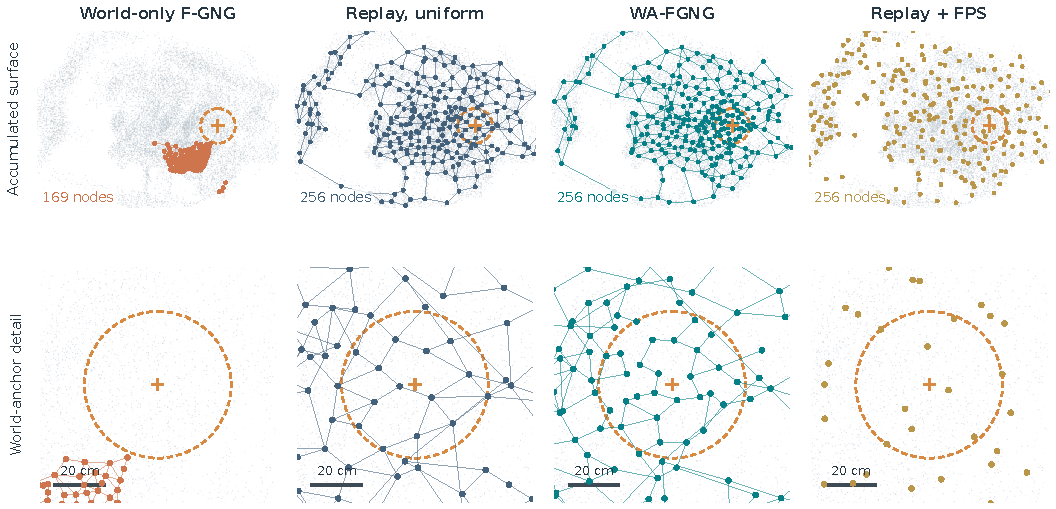
\includegraphics[width=\textwidth]{qualitative_desk.pdf}
\caption{Prespecified qualitative comparison on fr1/desk, selected frame 119, seed 1, node cap 256. Gray points are the causal held-out reference. All columns use the same world-coordinate orthographic projection onto the first camera's image axes; the bottom row magnifies the anchor region. Orange circles indicate the projected 0.30\,m attention scale, and crosses mark the world anchor. Current-frame learning concentrates on the latest view, while replay supports earlier surfaces. Foveation increases local prototype density relative to a constant attention field. FPS is a point-set comparison and has no learned edges. A projected circle does not imply that every enclosed point lies within the 3D focal sphere.}
\label{fig:qualitative}
\end{figure*}

\subsection{Focal Accuracy and Global Cost}
The matched uniform-field ablation is the relevant comparison for spatial attention: it shares the support memory, replay sequence, node cap, and reallocation gating. At $B=256$, foveation reduces mean focal error from \DeskUniformFocus{} to \DeskMemoryFocus{}\,cm on \texttt{desk} and from \XyzUniformFocus{} to \XyzMemoryFocus{}\,cm on \texttt{xyz}, improvements of \DeskFocusGain\% and \XyzFocusGain\%. Mean error over all observed surfaces increases by \DeskGlobalCost\% and \XyzGlobalCost\%, respectively. This is the intended redistribution trade-off: finite representational capacity is shifted toward the anchor at a measurable global cost.

The qualitative graph in Fig.~\ref{fig:qualitative} shows this redistribution, while the lower curves in Fig.~\ref{fig:temporal} expose behavior through the prescribed A--B--A schedule. The curves do not establish an optimal switching policy or a settling-time guarantee. The anchors are selected geometrically, without object labels, and the attention sequence is fixed independently of graph quality.

DBL-GNG with the same support achieves lower global error than \method{} on both primary sequences (\DeskDblSeen{} versus \DeskMemorySeen{}\,cm on \texttt{desk}; \XyzDblSeen{} versus \XyzMemorySeen{}\,cm on \texttt{xyz}), while \method{} achieves lower focal error. FPS yields focal errors of \DeskFpsFocus{} and \XyzFpsFocus{}\,cm with the same sample and output-point limits. These outcomes support targeted allocation as a trade-off, rather than dominance across all metrics. The budget sweep in Fig.~\ref{fig:cost} also makes clear that representation quality depends on the chosen node limit.

\begin{figure*}[t]
\centering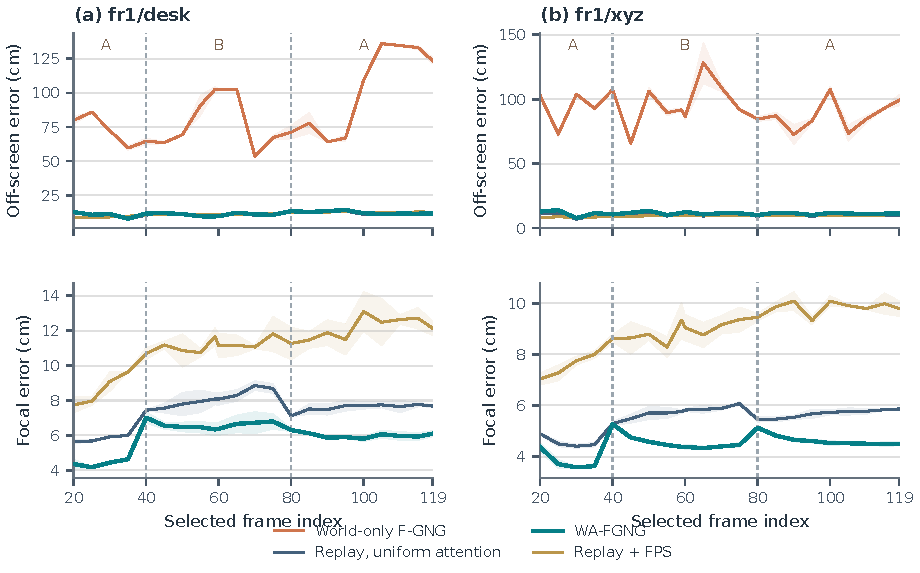
\includegraphics[width=\textwidth]{temporal_results.pdf}
\caption{Primary temporal results at $B=256$. Upper panels compare off-screen retention with and without historical replay. Lower panels compare focal accuracy among matched replay methods; the much larger world-only focal errors are reported in Table~\ref{tab:main} rather than compressing this plot's scale. Dashed vertical lines mark the prescribed attention switches at frames 40 and 80. Lines are means and shaded bands are sample standard deviations over three algorithm seeds on the same recorded sequence, not confidence intervals across environments.}
\label{fig:temporal}
\end{figure*}

\subsection{Graph Support and Update Cost}
Focal accuracy does not imply improved adjacency. The fraction of learned edges with an interior sample farther than 5\,cm from the observed reference is \DeskMemoryEdge{}\% for \method{} versus \DeskUniformEdge{}\% for the uniform-field ablation on \texttt{desk}; on \texttt{xyz}, these values are \XyzMemoryEdge{}\% and \XyzUniformEdge{}\%. DBL-GNG has lower values of \DeskDblEdge{}\% and \XyzDblEdge{}\%, respectively. This diagnostic reveals residual unsupported connections even when point-to-node coverage is useful. It should not be interpreted as a collision rate or an exact topological error rate.

At $B=256$, mean per-run 95th-percentile update times for \method{} are \DeskMemoryTime{}\,ms on \texttt{desk} and \XyzMemoryTime{}\,ms on \texttt{xyz}. Corresponding FPS values are \DeskFpsTime{} and \XyzFpsTime{}\,ms, while DBL-GNG values are \DeskDblTime{} and \XyzDblTime{}\,ms. These include world transformation, support updates, replay, learning, and graph extraction, but exclude depth decoding, pose estimation, and evaluation. The measurements describe this CPU implementation under its recorded execution conditions; they are not end-to-end sensor-to-action latency. Current-frame learning is faster but represents substantially less historical geometry.

\begin{figure*}[t]
\centering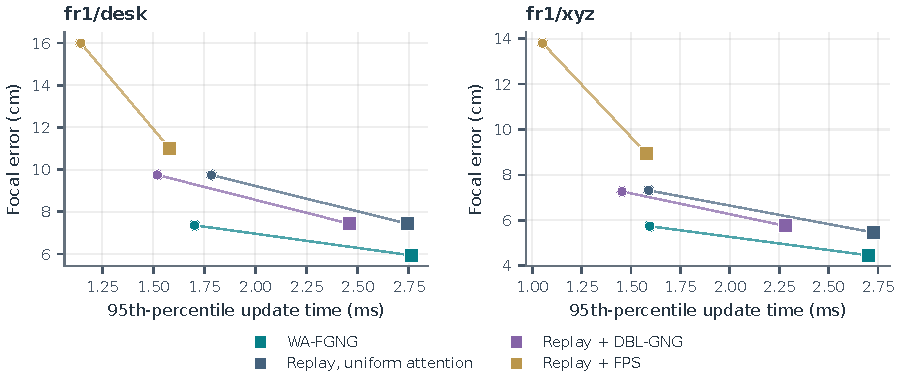
\includegraphics[width=\textwidth]{accuracy_cost.pdf}
\caption{Measured focal-error/update-cost trade-off among memory-based methods on the primary sequences. Circles denote a node cap of 128 and squares a cap of 256; lines connect the same method across the two caps. Each point averages three run summaries. The horizontal coordinate is the mean of per-run 95th-percentile update times. FPS is faster in these runs but allocates fewer samples to the prescribed focal region. CPU operating conditions were not fixed; small timing differences should not be overinterpreted.}
\label{fig:cost}
\end{figure*}

\subsection{Pose Perturbations and Additional Rotation Sequence}
A separate sensitivity test perturbs the supplied poses while keeping evaluation geometry and world anchors fixed. For each frame, independent Gaussian translation perturbations have per-axis standard deviation 0, 1, or 3\,cm; rotation-vector components have corresponding standard deviations 0, 1, or 3 degrees. Rotation is applied about the camera center. The same standardized perturbations are reused across severity levels for each seed. This tests artificial pose jitter, not the trajectory drift of a real SLAM system.

Across three seeds at $B=256$, mean accumulated-surface error on \texttt{desk} rises from \DeskPoseZeroSeen{}\,cm with oracle poses to \DeskPoseOneSeen{} and \DeskPoseThreeSeen{}\,cm at the two nonzero levels. On \texttt{xyz}, it rises from \XyzPoseZeroSeen{} to \XyzPoseOneSeen{} and \XyzPoseThreeSeen{}\,cm. Focal error rises from \DeskPoseZeroFocus{} to \DeskPoseOneFocus{} and \DeskPoseThreeFocus{}\,cm on \texttt{desk}, and from \XyzPoseZeroFocus{} to \XyzPoseOneFocus{} and \XyzPoseThreeFocus{}\,cm on \texttt{xyz}. The zero-noise runs exactly reproduce the corresponding primary accuracy summaries. Memory preserves supplied geometry; it cannot correct erroneous registration.

\begin{table}[t]
\centering\small
\caption{Additional rotation sequence, fr1/rpy, at $B=256$. Mean errors in cm across three seeds; same fixed protocol. This sequence was added after the two-sequence primary protocol was fixed.}
\label{tab:rotation}
\begin{tabular}{lrr}
\toprule Method & All observed & Focal \\
\midrule
Unregistered F-GNG & 103.93 & 52.60 \\
World-only F-GNG & 106.45 & 57.86 \\
\textbf{WA-FGNG} & 14.68 & 6.89 \\
Replay, uniform field & 14.39 & 9.11 \\
Replay + DBL-GNG & 13.44 & 9.03 \\
Replay + FPS & 15.10 & 14.36 \\
\bottomrule\end{tabular}
\end{table}

An additional fr1/rpy experiment uses the same parameters, node limit 256, and three seeds, yielding 18 further runs. Its 120 selected frames span 24.1\,s. As Table~\ref{tab:rotation} shows, foveation reduces focal error from \RpyUniformFocus{} to \RpyMemoryFocus{}\,cm relative to the matched uniform-field ablation, a \RpyFocusGain\% improvement, with a \RpyGlobalCost\% increase in global error. Unsupported-edge fraction remains \RpyMemoryEdge\% for \method{}. This adds evidence under rotational camera motion, while remaining within the benchmark's narrow office/sensor regime.



\section{Discussion and Limitations}
Replay and attention address different allocation problems. Persistent support improves historical coverage, while foveation trades global accuracy for focal detail; downstream requirements determine whether that trade-off is useful.

The experiment conditions on supplied poses. Calibration errors, pose drift, tracking failures, and loop-closure corrections can invalidate accumulated coordinates. The pose-jitter test quantifies one sensitivity, but does not reproduce the correlated errors of a real tracker. Disjoint reference pixels share the sensor and pose source and are not independent surveyed geometry.

Memory assumes a static scene and has no visibility-based removal. Hash retention bounds and stabilizes support cardinality, but can evict rare or task-relevant surfaces. The positive attention floor gives no minimum coverage guarantee. Split--merge thresholds remain heuristic, prototype IDs do not identify physical surface points, and unsupported edges persist. The graph consequently cannot be treated as a certified collision or traversability model.

ROI-GNG, the closest attention-based alternative, is not included as an executable baseline. Comparative conclusions are restricted to the matched ablations, DBL-GNG, and FPS. The Freiburg 1 office recordings cover a narrow environment and sensor regime; rpy expands camera-motion coverage rather than scene diversity. Estimated trajectories, dynamic scenes, task-derived attention, and closed-loop robot experiments are needed to assess broader utility.

\section{Conclusion}
World-anchored replay sustains historical graph support, while spatial attention reallocates resolution toward a selected region at a measurable global cost. Separate support, replay, and graph budgets make these effects testable through controlled comparisons. The accompanying data provenance, executable outputs, and plotting scripts support reproduction of this known-pose representation study.

\section*{Acknowledgments and AI Disclosure}
OpenAI Codex assisted with manuscript text throughout, mapping and benchmark code in Sections III--IV, and figure/table scripts. Experimental values and plots derive from recorded inputs and executable outputs. The architecture drawing is a labeled schematic.

\bibliographystyle{IEEEtran}
\bibliography{references}
\end{document}
